%!TEX root = ../thesis.tex

\chapter{Background}\label{ch:background}
In this chapter, we provide the theoretical background required for this thesis, most notably introducing the flow map of a deterministic system and building up to It\^o stochastic differential equations as a means of incorporating uncertainty into these models.
Further details, including some of the technical results and tools employed later, and provided in \Cref{app:theory}.
The chapter is concluded by summarising stochastic sensitivity \citep{Balasuriya_2020_StochasticSensitivityComputable}, which provided initial tools for characterising uncertainty in a computationally efficient manner and is the primary motivation for this work.

% In this chapter, we first motivate the need for stochastic models with a simple example predicting the path of a drifter in the Gulf Stream.o

% Throughout, we will use an example of tracking a drifter in the Gulf Stream to illustrate the concepts introduced.
% We will return to this example in more detail, including applying our later developments, in \Cref{ch:appls}.

% We then briefly review the current literature on stochastic parameterisation, which is the introduction of stochastic terms into otherwise deterministic models, in the context of atmospheric modelling, oceanography and climate forecasting.
% Finally, we highlight the limitations of bulk stochastic simulation as a means of working with complicated stochastic models, both in terms of computational costs and accuracy.
% This suggests the need, across a variety of applications, for developing computationally efficient methods for approximating prediction distributions of such stochastic models, which this thesis aims to address.


\section{Notation}
We start this chapter by introducing the mathematical notation that will be used throughout this thesis.
The set of \(n \times m\) matrices with real-valued entries is denoted as \(\R^{n\times m}\).
% In general, the \(i\)th component of a vector \(x\) is denoted by \(x_{i}\), except where there is already a subscript, in which case we write \(x_t^{(i)}\) to denote the \(i\)th component of \(x_t\), for instance.
% For a matrix \(A\), \(\left[A\right]_{\cdot i}\) typically refers to the \(i\)th column, and \(\left[A\right]_{i\cdot}\) the \(i\) the row of \(A\).
The norm symbol \(\norm{\cdot}\) without any additional qualifiers denotes the standard Euclidean norm for a vector, and the spectral (operator) norm induced by the Euclidean norm, i.e. for an \(n \times n\) matrix \(A\)
\[
	\norm{A} = \sup\left\{\frac{\norm{Av}}{\norm{v}}\,\middle|\,v \in \R^n, \, \norm{v} \neq 0\right\}.
\]

For a random variable \(X\), we use \(\avg{X}\) to denote the expectation of \(X\) and \(\var{X}\) to denote the variance.
For a \(n\)-dimensional vector-valued random variable \(Y\), \(\avg{Y}\) again denotes the (now vector-valued) expectation of \(Y\), and \(\var{Y}\) denotes the covariance matrix of \(Y\).
That is, \(\var{Y}\) is the \(n\times n\) matrix with \((i,j)\)th component
\[
	\left[\var{Y}\right]_{ij} = \avg{Y_iY_j} - \avg{Y_i}\avg{Y_j} = \cov{Y_i, Y_j} = \begin{cases}
		\var{Y_i},      & \text{if } i = j, \\
		\cov{Y_i, Y_j}, & \text{otherwise},
	\end{cases}
\]
where \(\cov{Y_i, Y_j} = \avg{\left(Y_i - \avg{Y_i}\right)\left(Y_j - \avg{Y_j}\right)}\) denotes the (scalar) covariance between \(Y_i\) and \(Y_j\).

There are several different notions of convergence for a sequence of random variables, which we briefly recall here.
Consider a sequence of \(m\)-dimensional random vectors \(X_1, X_2,\dotsc\) and an \(m\)-dimensional random vector \(X\).
We say that:
\begin{itemize}
	\item The sequence \(X_1, X_2, \dotsc\) converges \emph{in distribution} to \(X\) if
	      \[
		      \lim_{n\to\infty}F_n\left(x\right) = F(x),
	      \]
	      where \(F_n\) is the cumulative distribution function for \(X_n\) and \(F\) is the cumulative distribution function for \(X\), for every point \(x \in \R^m\) where \(F\) is continuous.
	      If this is the case, we write
	      \[
		      X_n \xlongrightarrow[\text{distribution}]{} X, \quad \text{as } n \to \infty.
	      \]
	      Note that the limiting random vector \(X\) need not be defined on the same probability space as the terms in the sequence \(X_1, X_2, \dotsc\); convergence in distribution is the only notion of convergence for which this is the case.


	\item The sequence \(X_1, X_2, \dotsc\) converges \emph{in probability} to \(X\) if for every \(\delta > 0\)
	      \[
		      \lim_{n\to\infty}P\left(\norm{X_n - X} < \delta\right) = 0,
	      \]
	      in which case we write
	      \[
		      X_n \xlongrightarrow[\text{probability}]{} X, \quad \text{as } n \to \infty.
	      \]

	\item The sequence \(X_1, X_2, \dotsc\) converges \emph{almost surely} to \(X\) if
	      \[
		      P\left(\lim_{n \to \infty}X_n = X\right) = 1,
	      \]
	      in which case we write
	      \[
		      X_n \xlongrightarrow[\text{almost surely}]{} X, \quad \text{as } n \to \infty.
	      \]

	\item For \(r > 0\), the sequence \(X_1, X_2, \dotsc\) converges \emph{in \(r\)th mean} to \(X\) if
	      \[
		      \lim_{n\to\infty}{\avg{\norm{X_n - X}^r}} = 0,
	      \]
	      in which case we write
	      \[
		      X_n \xlongrightarrow[r\text{th mean}]{} X, \quad \text{as } n \to \infty.
	      \]
	      This type of convergence is also known as \emph{\(L_r\)-convergence}, as it corresponds to convergence in the \(L_r\) norm on the probability space on which \(X_1,\dotsc, X_n\) and \(X\) are defined.

\end{itemize}
There are implications between each notion of convergence, with convergence almost surely being the strongest and convergence in distribution the weakest.
These implications are summarised in \Cref{fig:rv_conv_impl}.

\usetikzlibrary{positioning}
\begin{figure}
	\begin{center}
		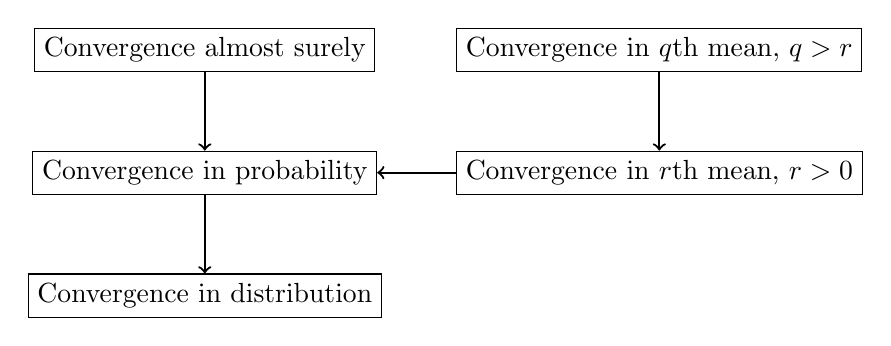
\begin{tikzpicture}
			\node (as) [draw] {Convergence almost surely};
			\node (p) [draw, below=of as] {Convergence in probability};
			\node (rm) [draw, right=of p] {Convergence in \(r\)th mean, \(r > 0\)};
			\node (qm) [draw, above=of rm] {Convergence in \(q\)th mean, \(q > r\)};
			% \node (rmom) [draw, below=of rm] {Convergence of \(r\)th moment};
			\node (d) [draw, below=of p] {Convergence in distribution};
			\path[->,thick] (as) edge  (p)
			(p) edge  (d)
			(qm) edge (rm)
			(rm) edge (p);
			% (rm) edge (rmom);
		\end{tikzpicture}
		\caption{The strength of each notion of convergence in probability, where each directed arrow corresponds to an implication.
			These results are stated and proven in \citet{Bremaud_2020_ProbabilityTheoryStochastic}, for instance.}
		\label{fig:rv_conv_impl}
	\end{center}
\end{figure}






\section{The flow map}
Ordinary differential equations are used to model many different phenomena across a range of fields and applications.
Specifically, the continuous time evolution of a multi-dimensional state variable is governed by a system of first order differential equations of the form
\begin{equation}\label{eqn:det_ode}
	\dod{w_t}{t} = u\!\left(w_t, t\right),
\end{equation}
where \(w_t \in \R^n\) is the time-evolving variable of interest and \(u\) is the vector field specified at each relevant state and time \(t\).
The vector field \(u\) may be derived from a specified model, or may be driven or supplemented by observed data.
Since data has a finite-time limitation, we typically consider the evolution of \cref{eqn:det_ode} over a finite time interval \([0,T]\).
In this thesis, we restrict ourselves to the finite time setting.
We can solve \cref{eqn:ode_det} analytically, or, as is often required in practice, numerically to generate time evolving trajectories, which can inform future predictions or be used to reconstruct past behaviour.
% The solutions to the differential equations of the form \cref{eqn:det_ode} define a continuous-time dynamical system.
The flow map of \cref{eqn:det_ode} provides a convenient way of summarising the trajectories that solve \cref{eqn:det_ode} and working with these solutions analytically.
Formally, the flow map \(F_{s}^{t}: \R^n \to \R^n\) from time \(s\) to \(t\) associated with \cref{eqn:det_ode} is the unique solution to
\begin{equation}
	\dpd{F_{s}^{\tau}\!\left(x\right)}{\tau} = u\left(F_{s}^\tau\!\left(x\right), \tau\right), \qquad F_{s}^{s}\!\left(x\right) = x,
	\label{eqn:flow_map_ode}
\end{equation}
solved up to time \(\tau = t\).
That is, the flow map is the operator mapping initial conditions at time \(t\) to their corresponding positions at time \(s\), under the continuous-time evolution of \cref{eqn:det_ode}.
\td{Possibly add a diagram showing the flow map, but not sure yet whether this would add anything.}
% \Cref{fig:flow_map} provides a pictorial representation of the flow map; .
Equivalently, the flow map satisfies the integral form of \cref{eqn:det_ode}:
\begin{equation}\label{eqn:flow_map_int}
	F_s^t\!\left(x\right) = x + \int_s^t{u\!\left(F_s^{\tau}\!\left(x\right), \tau\right)\dif \tau}.
\end{equation}
We use the flow map to represent all solutions of the deterministic differential equation \cref{eqn:det_ode}, with the understanding that for any relevant initial condition, the flow map at that point can be readily computed by solving the ODE either analytically or numerically.
We view the flow map primarily as a function of the initial condition, so that it quantifies the impa8ct of 8changes in the initial condition on future predictions.
Accordingly, the gradient \(\nabla F_s^t\) of the flow map (with respect to the initial condition) provides insight into the local behaviour of the dynamical system \citep{Arnold_1973_OrdinaryDifferentialEquations,TruesdellNoll_2004_NonLinearFieldTheories}.
For any times \(s, t \in [0,T]\), this gradient	\(\nabla F_s^t\) satisfies a useful property:
\begin{equation}
	\dpd{\nabla F_{s}^{t}\!\left(x\right)}{t} = \nabla u\!\left(F_{s}^{t}\!\left(x\right), t\right) \nabla F_{s}^{t}\!\left(x\right),
	\label{eqn:eqn_of_variations}
\end{equation}
which is the equation of variations corresponding to \cref{eqn:det_ode}.
This result can be shown by taking the gradient of both sides in \cref{eqn:flow_map_ode} and using the chain rule.




\section{From ODEs to SDEs}
Differential equations are well-studied and ubiquitously employed across many fields.
These models are \emph{deterministic}, in that given an initial condition an ODE provides a single prediction of the future state.
However, in practice any such model will be subject to unavoidable uncertainty, which can arise from a range of sources including but not limited to:
\begin{itemize}
	\item observational errors in any measured data used to construct the model,
	\item uncertainty in any parameters involved in the model,
	\item unexplainable phenomena not captured by the model,
	\item numerical errors in the discretisation of the model, and
	\item uncertainty in the knowledge of the initial state.
\end{itemize}
By accounting for any of these in our model, we expect to improve the power and accuracy of our predictions.
However, the true nature of this uncertainty is unknowable, so it is common to model it as a random process.
That is, we extend our deterministic model to a \emph{stochastic} one, where the solution (and therefore our predictions of the future state) is now a random variable.
There are several approaches to establishing such a framework, the most general of which is a random dynamical system \citep{Arnold_1998_RandomDynamicalSystems,NeckelRupp_2013_RandomDifferentialEquations}.
However, when working in a continuous-time and continuous-state modelling scenario, a natural extension of an ordinary differential equation to account for this uncertainty is a stochastic differential equation (SDE).
Although an SDE is an ``improvement'' over the deterministic ODE, in the sense that uncertainty can be encoded in the model itself, the compromise is that solutions are no longer straightforward to obtain or even analyse.
In fact, the formal treatment of SDEs requires an entirely new notion of integration, as we shall discuss.
Nonetheless, SDEs provide a rich framework for modelling and are used as predictive tools in a range of applications and fields \citep{Balasuriya_2020_StochasticApproachesLagrangian,SarkkaSolin_2019_AppliedStochasticDifferential,Oksendal_2003_StochasticDifferentialEquations,Jazwinski_2014_StochasticProcessesFiltering}, most notably financial mathematics \citehere, weather and climate modelling \citep{BernerEtAl_2017_StochasticParameterizationNew,Palmer_2019_StochasticWeatherClimate,FranzkeEtAl_2015_StochasticClimateTheory}.
For a formal introduction to stochastic differential equations, see \citet{Oksendal_2003_StochasticDifferentialEquations} or \citet{KallianpurSundar_2014_StochasticAnalysisDiffusion}, for instance.
There are several different ways to construct stochastic differential equations from deterministic dynamics; the following motivation of stochastic differential equations loosely follows a similar one available in \citet{Oksendal_2003_StochasticDifferentialEquations}, but other formulations of SDEs are available, e.g. using rough path theory \citep{FrizVictoir_2010_MultidimensionalStochasticProcesses}.

Suppose that we have a deterministic ordinary differential equation, i.e. \cref{eqn:ode_det}, and aim to account for uncertainty in the vector field \(u\).
In lieu of any additional understanding of this uncertainty, we model it as a stochastic noise.
Ideally, we would parameterise the uncertainty with some continuous-time stochastic process \(\xi_t\!\left(x_t\right)\), and write
\[
	\dod{y_t}{t} = u\left(x_t, t\right) + \xi_t\!\left(x_t\right).
\]
The noise process \(\xi_t\) can depend on the state, since we may expect that the magnitude and structure of the uncertainty varies with both the state and time.
In most modelling situations, we expect that the noise process \(\xi_t\) should have the properties:
\begin{enumerate}
	\item For any two distinct times \(s \neq t\), the random variables \(\xi_s\) and \(\xi_t\) are independent.
	\item The process is stationary, that is the joint distribution of \(W_{t_1 + t}, \dotsc, W_{t_k + t}\) does not depend on \(t\).
	\item For all \(t\), \(\avg{\xi_t} = 0\).
\end{enumerate}
Additionally, since we are modelling with a continuum, the noise process \(\xi_t\) should be (with probability \(1\)) continuous in time.
However, such a noise process \(\xi_t\) does not exist \citep{Oksendal_2003_StochasticDifferentialEquations}, in that there is no  continuous process with properties 1 to 3, so we need an alternative formulation of the integral.
This leads to the It\^o integral, and It\^o stochastic differential equations, which we introduce in \Cref{sec:bkg_ito} and \Cref{sec:bkg_sde} respectively.



\subsection{The Wiener process}


In the absence of any additional knowledge about the nature of the noise (such as skew), the canonical Wiener process is the standard choice.
Defined formally, the (one-dimensional) canonical \emph{Wiener process} is a stochastic process \(B_t\) taking values in \(\R\) and satisfying the following properties:
\begin{romanate}
	\item \(B_0 = 0\),
	\item for every \(s > 0\), the increments \(B_{s + t} - B_{s}\) for \(t \geq 0\) are independent of \(B_r\) for all \(r < s\),
	\item \(B_{s + t} - B_t \isGauss{0, s}\) for all \(s,t > 0\), and
	\item \(B_t\) is continuous in \(t\) almost surely.
\end{romanate}
Remarkably, these properties \emph{uniquely} define the Wiener process, with the additional result that for any \(t > 0\), \(B_t \sim \mathcal{N}\left(0, t\right)\), a Gaussian distribution with mean zero and variance \(t\).
The \emph{\(n\)-dimensional Wiener process} is a stochastic process \(W_t\) taking values in \(R^n\) such that each component of \(W_t\) is a one-dimensional Wiener process and the components of \(W_t\) are mutually independent.
It follows that for the \(n\)-dimensional Wiener process \(W_t\), at any time \(t > 0\), \(W_t \sim \mathcal{N}\left(0, tI\right)\), an \(n\)-dimensional Gaussian distribution with mean zero and covariance matrix \(tI\).
\Cref{fig:wiener_rels} plots realisations of a one-dimensional and two-dimensional Wiener process.

\begin{figure}
	\begin{center}
		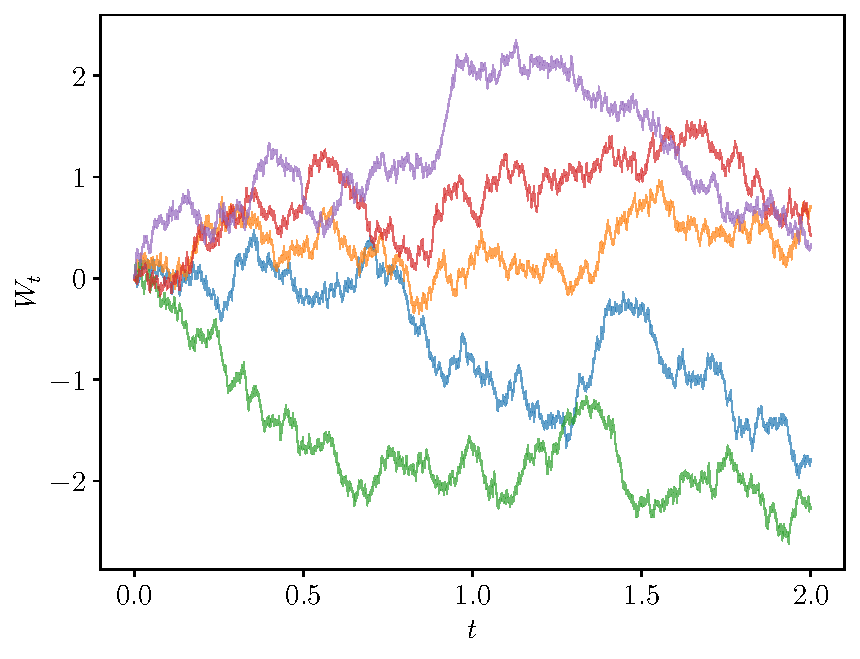
\includegraphics[width=0.49\textwidth]{figures/wiener_realisations_1d.pdf}
		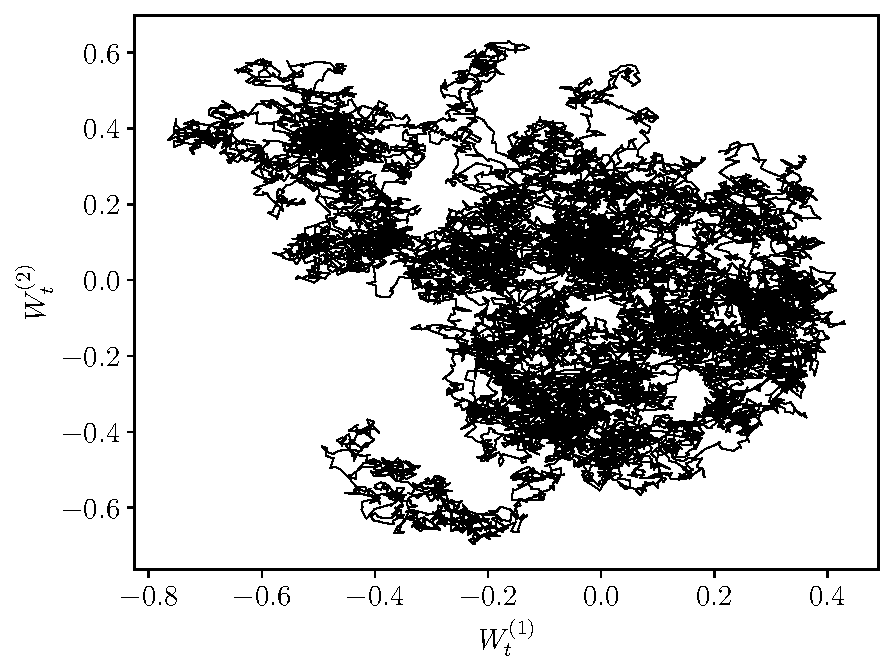
\includegraphics[width=0.49\textwidth]{figures/wiener_realisations_2d.pdf}
		\caption{(Left) Several realisations of a one-dimensional Wiener process \(W_t\) evolving through time, and (right) a realisation of two-dimensional Wiener process \(\left(W_t^{(1)}, W_t^{(2)}\right)\).}
		\label{fig:wiener_rels}
	\end{center}
\end{figure}


\subsection{The It\^o integral}\label{sec:bkg_ito}
The non-differentiability of the Wiener process means that standard deterministic calculus is not sufficient to introduce continuous-time uncertainty into a differential equation.
Instead, this lead to an entirely new definition of the integral by \citet{Ito_1944_StochasticIntegral,Ito_1946_StochasticIntegralEquation} that enabled integration with respect to a broad class of stochastic processes.
For our purposes, we can think of an It\^o integral as being defined as the limit in probability of a sequence of sums, i.e. for a scalar but possibly random-valued function \(f\colon [a,b] \to \R\),
\begin{equation}\label{eqn:ito_int_limit_defn}
	\sum_{\left[t_i, t_{i+1}\right] \in \mathcal{P}_N}{f\left(t_{i}\right)\left(W_{t_{i+1}} - W_{t_i}\right)} \xlongrightarrow[\text{probability}]{} \int_a^b{f(t)\dif W_t}, \quad \text{as } N \to \infty
\end{equation}
where \(\mathcal{P}_N\) is a partition of \(\left[a,b\right]\) with \(\lim_{N \to \infty}\mathcal{P}_N = [a,b]\), \emph{\`a la} the definition of the Riemann integral.
It can be shown (see the textbooks by \citet{KallianpurSundar_2014_StochasticAnalysisDiffusion} and \citet{Oksendal_2003_StochasticDifferentialEquations}, for instance) that this limit exists for a large class of both deterministic- and random-valued functions, by constructing appropriate approximations of the function \(f\).

The extension of the It\^o integral to vector- and matrix-valued functions is straightforward.
Let \(g \colon [a,b] \to \R^{n \times m}\) be a function giving possibly random \(n \times m\) matrices (take \(m = 1\) to describe a vector-valued function).
\begin{subequations}\label{eqn:mv_ito_defn}
	Then, we define the It\^o integral of \(g\) with respect to the \(m\)-dimensional Wiener process \(W_t\) over the time interval \([a,b]\) as
	\begin{equation}\label{eqn:mv_ito_defn_1}
		\int_a^b{g(t)\dif W_t} \coloneqq \left(\mathcal{I}_1, \dotsc, \mathcal{I}_n\right)^{\T},
	\end{equation}
	where
	\begin{equation}\label{eqn:mv_ito_defn_2}
		\mathcal{I}_{i} = \sum_{j=1}^m{\int_a^b{g_{ij}\left(t\right) \dif W_t^{(j)}}},
	\end{equation}
	for \(i = 1,\dotsc, n\) and where \(g_{ij}\) denotes the \((i,j)\)th element of \(g\).
\end{subequations}


\subsection{It\^o stochastic differential equations}\label{sec:bkg_sde}
Equipped with the It\^o integral as a formal definition of an integral with respect to a stochastic process, we can now extend the notion of an ordinary differential equation to include stochasticity.
The differential form of an \(n\)-dimensional It\^o stochastic differential equation is
\begin{equation}
	\dif y_t = u\!\left(y_t, t\right)\dif t + \sigma\!\left(y_t, t\right)\dif W_t,
	\label{eqn:gen_sde}
\end{equation}
where the solution \(y_t\) is a stochastic process taking values in \(\R^n\), \(u\colon \R^n \times \R \to \R^n\) is the drift and \(\sigma\colon \R^n \times \R \to \R^{n\times m}\) is the diffusivity.
The driving process \(W_t\) is the \(m\)-dimensional Wiener process.
The notation in \cref{eqn:gen_sde} is not rigorously defined (the solution \(y_t\) is not differentiable in general, for example), but rather taken as equivalent to the integral form
\begin{equation}
	y_t = y_0 + \int_0^t{u\left(y_\tau, \tau\right)\dif\tau} + \int_0^t{\sigma\left(y_\tau, \tau\right)\dif W_\tau}.
	\label{eqn:gen_sde_int}
\end{equation}
where \(y_0\) is the possibly random initial condition.
In the most general case, the drift \(u\) and diffusivity \(\sigma\) are permitted to themselves be random function%s\footnote{For more information, see for instance \citet{KallianpurSundar_2014_StochasticAnalysisDiffusion}.
% The formal treatment of such stochastic differential equations remains an area of open research, such as establishing the conditions for existence and uniqueness of solutions \citehere, and EXAMPLE.}
, but in this thesis we assume that both are deterministic.

The nature of the noise is characterised by the diffusion matrix \(\sigma\).
When \(\sigma\) does not depend on the solution \(y_t\), the noise is termed \emph{additive}, whereas if \(\sigma\) does depend on the solution, then the noise is \emph{multiplicative}.
SDEs with additive noise are typically easier to solve and analyse than those with multiplicative noise, but multiplicative noise is often required in practice to capture uncertainty that varies with state.

There are many analytic tools available for working with stochastic differential equations, such as It\^o's Lemma, an analogy of the chain rule.
The results that are used in this thesis (most notably the proofs presented in \Cref{ch:linear_theory}) are summarised in \Cref{app:ito_tools}.

% \begin{figure}
% 	\begin{center}
% 		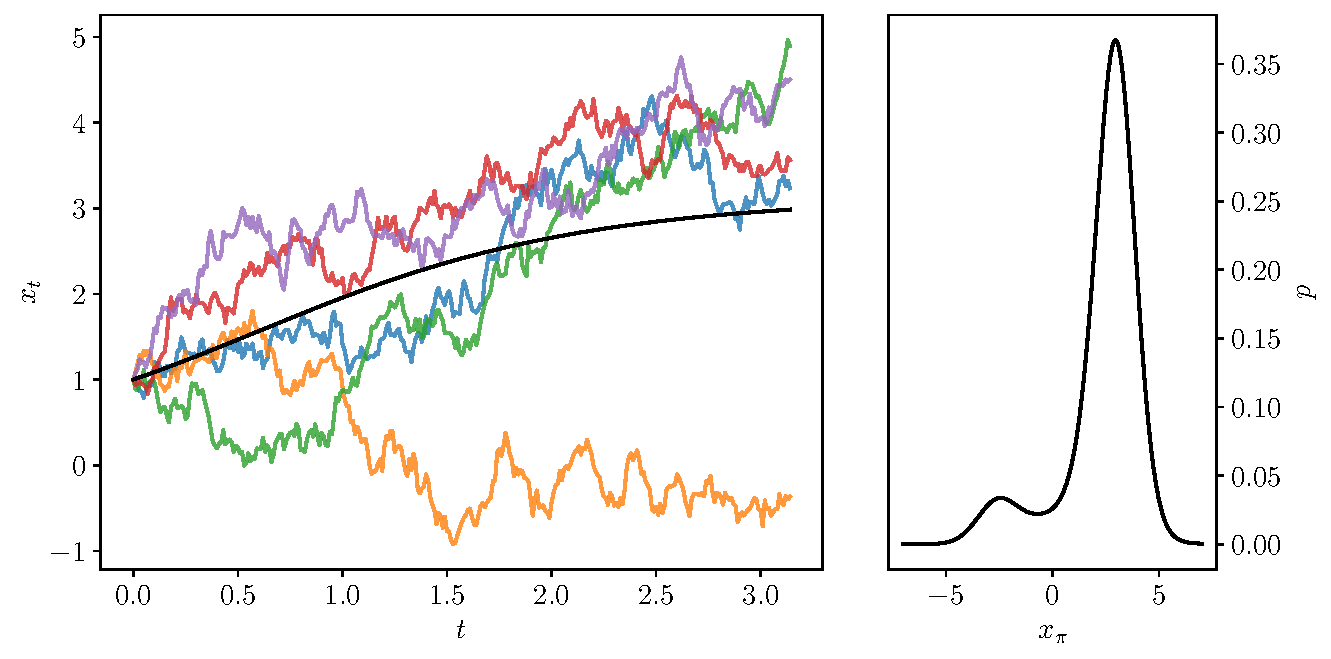
\includegraphics[width=\textwidth]{figures/ou_solution.pdf}
% 		\caption{Sample paths of the solution to the stochastic differential equation \(\dif x_t = \sin\!\left(x_t\right)\dif t + \dif W_t\), from the initial condition \(x_0 = 1\) and over the time interval \((0,\pi)\).
% 			The solution to the corresponding deterministic system is in black with the same initial condition is in black.}
% 		\label{fig:sde_sol_sample}
% 	\end{center}
% \end{figure}

% As an example, in \Cref{fig:sde_sol_sample} we show 10 stochastic samples of the solution to the SDE \(\dif x_t = \sin\!\left(x_t\right)\dif t + \dif W_t\).
% The corresponding deterministic system
% Two trajectories (the blue and orange) deviate from the behaviour of the deterministic system.



% Stochastic differential equations also arise as the limit of deterministic slow-fast systems, where the average behaviour of the `fast' dynamics can be shown to converge to the solution of a stochastic differential equation \citep[e.g.]{WongZakai_1965_ConvergenceOrdinaryIntegrals,MelbourneStuart_2011_NoteDiffusionLimits,GottwaldMelbourne_2013_HomogenizationDeterministicMaps}\lb{Maybe some better citations out there.}.
% A review of this theory is provided by \citet{GivonEtAl_2004_ExtractingMacroscopicDynamics}.
% This is particular relevant in climate and physics applications, where \citep{FranzkeEtAl_2015_StochasticClimateTheory}.
% This leads to stochastic parameterisation \citep{BernerEtAl_2017_StochasticParameterizationNew,Palmer_2019_StochasticWeatherClimate}, which we review in more detail in \Cref{sec:stoch_param}.

The noise driving stochastic differential equations need not be a Wiener process, and can be instead replaced by any semi-martingale, which are a general class of stochastic processes.
However, we primarily use the Wiener process throughout this thesis due to the aforementioned properties that make it appropriate for modelling scenarios and the ubiquitous use of it across literature and applications.
We do briefly discuss the possibility of extending some of our work to L\'evy processes, a  more general class of stochastic processes, in \Cref{sec:disc_levy}.



\subsection{Numerical schemes for approximating SDEs}
In general, solving a stochastic differential equation analytically is not possible, and so as with ordinary differential equations we instead look to use numerical schemes to approximate solutions.
However, the solution to a stochastic differential equation is itself a random variable, so a single sample path is not sufficient.
Instead, a numerical SDE scheme involves random sampling (typically of the driving noise process) and produces approximate \emph{realisations} of the solution.
With a large number of these Monte-Carlo realisations, one can estimate statistical properties and approximate the distribution of the solution.
The stochastic sampling approach is the gold-standard in many applications, most notably climate and weather modelling \citep{Collins_2007_EnsemblesProbabilitiesNew},  where complicated stochastic models cannot be used analytically.

The simplest scheme for numerically solving SDEs is the Euler-Maruyama (EM) method, which is analogous to the Euler method for ODEs \citep{KloedenPlaten_1992_NumericalSolutionStochastic}.
The update step of the EM scheme, with step size \(\delta t\), is
\begin{equation}
	\hat{x}_{t + \delta t} = \hat{x}_{t} + \Delta t u\!\left(\hat{x}_t, t\right) + \delta t \sigma\!\left(\hat{x}_t, t\right) Z_t,
	\label{eqn:em_step}
\end{equation}
where \(Z_t\) is sampled from the standard Gaussian \(\Gauss{0,I}\), and the scheme is initialised as \(\hat{x}_0 = x_0\).
% The Euler-Maruyama scheme has strong order 0.5, meaning that
% \[
% 	\avg{\norm{x_t - \hat{x}_{t}\left(\Delta t\right)}} = \mathcal{O}\left(\Delta t^{0.5}\right),
% \]
% where \(\hat{x}_t\left(\Delta t\right)\) is the Euler-Maruyama estimate at time \(t\) using step size \(\Delta t\).
There are many other schemes for generating approximate samples of a stochastic differential equation, of varying precision and computational efficiency, many of which are given in \citet{KloedenPlaten_1992_NumericalSolutionStochastic}.






\subsection{The Fokker-Planck equation}\label{sec:fp_eqn}
The Fokker-Planck (FP) equation is a partial differential equation that describes the time evolution of the probability density function of the solution to a stochastic differential equation.
The probability density function \(\rho: \R^n \times [0,T] \to [0,\infty)\) for the solution to \cref{eqn:gen_sde} at time \(t \in [0,T]\) is the solution to the corresponding Fokker-Planck equation \citep{Risken_2012_FokkerPlanckEquationMethods}
\begin{equation}
	\dpd{\rho}{t} = \frac12\nabla\cdot\nabla\cdot\left(\rho\sigma\sigma^{\T}\right) - \nabla\cdot\left(\rho u\right)
	\label{eqn:fp_eqn}
\end{equation}
subject to some initial density \(\rho\left(x,0\right)\) given by the initial condition to \cref{eqn:gen_sde}.
For a fixed and deterministic initial condition \(y_0 = x\), the corresponding initial condition to \cref{eqn:fp_eqn} is the Dirac-delta distribution centred at \(x\).
To ensure that the solution is a valid probability density function on \(\R^n\), for any \(t \in [0,T]\), \(\rho\) must satisfy
\begin{subequations}\label{eqn:fp_valid_pdf}
	\begin{align}
		\int_{\R^n}{\rho\left(x, t\right)\dif x} = 1, \label{eqn:fp_valid_pdf_norm} \\
		\lim_{x \to \infty}\rho\left(x,t\right) = 0. \label{eqn:fp_valid_pdf_limit}
	\end{align}
\end{subequations}
Solving the Fokker-Planck equation provides an alternative method for finding the solution to a stochastic differential equation; rather than dealing with stochastic quantities, we instead seek solutions to the
However, the Fokker-Planck equation cannot be solved analytically except for simple cases and there are several practical difficulties in attempting to solve it numerically.
These difficulties include:
\begin{itemize}
	\item \textbf{Dimensionality:} In high-dimensional systems, solving the Fokker-Planck equation numerically is computationally prohibitative, requiring a small spatial discretisation to be accurate.
	\item \textbf{Boundary conditions:} The Fokker-Planck equation is often defined on an unbounded domain with the zero-limit constraint \cref{eqn:fp_valid_pdf_limit}, which presents computational difficulties.
	\item \textbf{Normality constraints:} The Fokker-Planck equation must be solved with the additional normality condition \cref{eqn:fp_valid_pdf_norm}, which enforces an additional constraint on any numerical solution.
\end{itemize}
It is generally accepted that these difficulties mean that the computational cost of solving the Fokker-Planck equation is too high in \(3\)- or higher dimensions \citep{ZhaiEtAl_2022_DeepLearningMethod,Li_2019_DatadrivenMethodSteady,AllawalaMarston_2016_StatisticsStochasticallyForced}.

\td{Perhaps comment on how the FP equation arises in other settings, and is a generalisation of the advection-diffusion equation and similar. Hence learning stuff about the solution to the SDE also tells us about the FP equation.}

% \subsubsection{Relationship to the classical advection-diffusion equation}
% The advection-diffusion equation describes the time-evolution of a passive and inert scalar quantity, such as temperature, salinity

% \citep{Visser_2008_LagrangianModellingPlankton}

% Let \(c \colon \Omega_0 \times [0,T] \to [0, \infty)\) denote the concentration of a passive and inert scalar quantity, then the classical advection-diffusion equation is
% \begin{equation}\label{eqn:advec_diff}
% 	\dpd{c}{t} = - \nabla\cdot \left(v\!\left(x,t\right)c\!\left(x,t\right)\right) + \nabla\cdot\left(K\!\left(x,t\right)\nabla c\!\left(x,t\right)\right), \quad c\!\left(x,0\right) = c_0\!\left(x\right),
% \end{equation}
% where \(v\) denotes the flow velocity dictating the advection (displacement) of the tracer, and \(K\) is a matrix describing the diffusion (dispersion) of \(c\).




% If we set \(u\!\left(x,t\right) = v\!\left(x,t\right) + \nabla \cdot K\!\left(x,t\right)\) and \(\sigma\!\left(x,t\right)\sigma\!\left(x,t\right) = K\!\left(x,t\right)\), then the Fokker-Planck equation \cref{eqn:fp_eqn} is equivalent to the advection-diffusion equation \cref{eqn:advec_diff}.
% Thus, the evolution of the tracer concentration under \cref{eqn:advec_diff} can be equivalently considered as the probability density function of solutions to the stochastic differential equation
% \begin{equation}\label{eqn:ad_sde}
% 	\dif x_t = \left[u\!\left(x_t, t\right) + \nabla \cdot K\!\left(x_t, t\right)\right]\dif t + \kappa\!\left(x_t, t\right)\dif W_t, \quad x_t \sim \hat{c}_0,
% \end{equation}
% where \(\kappa\) is any matrix-valued function satisfying \(K \equiv \kappa\kappa^{\T}\), and
% \[
% 	\hat{c}_0\!\left(x\right) = \frac{c_0\!\left(x\right)}{\int_{\Omega_0}c_0\!\left(z\right)\dif z},
% \]
% is the initial density of \cref{eqn:advec_diff} normalised to describe a probability density function.
% Assuming that the total concentration tracer is conserved, that is
% \[
% 	\int_{\Omega_t}{c\!\left(z,t\right)\dif z} = \int_{\Omega_0}{c_0\!\left(z\right)\dif t}
% \]
% for all \(t \in [0,T]\), then we can recover \(c\) from the probability density function \(\rho\) corresponding to \cref{eqn:ad_sde} as
% \[
% 	c\!\left(x,t\right) = \rho\!\left(x,t\right)\int_{\Omega_0}{c_0\!\left(z\right)\dif t}.
% \]
% An implication of this connection is that the theory and computations for stochastic differential equations developed throughout this thesis can be applied to \emph{any} scalar field that is modelled with an advection-diffusion type equation.


% \subsubsection{Green's function method}
% The Fokker-Planck equation is linear, so we can apply a technique known as Green's function method (for an example of this approach on a linear SDE, see Section 3.2 of \citet{Risken_2012_FokkerPlanckEquationMethods}) in order to understand the behaviour of solutions with non-fixed initial conditions.
% Let \(\mathcal{P}_t\set{\rho_0}\) denote the solution operator of \cref{eqn:fp_eqn} with initial density \(\rho_0\colon \R^n \to \R^n\).
% Then, since \cref{eqn:fp_eqn} is a linear equation, \(\mathcal{P}_t\) is a linear operator.
% Now, let \(x_0 \in \R^n\) be an arbitrary fixed point, and consider the fundamental solution, or Green's function,
% \[
% 	G_t\left(x; x_0\right) \coloneqq \mathcal{P}_t\set{\delta_{x_0}}\!\left(x\right).
% \]
% That is, \(G_t\left(x; x_0\right)\) is the solution to the Fokker-Planck equation with the Dirac-delta initial condition \(\delta_{x_0}(x) = \delta\left(x - x_0\right)\), which is equivalent to the SDE \cref{eqn:gen_sde} with the deterministic and fixed initial condition \(y_0 = x_0\).
% The Green's function \(G_t\) is equivalently the transition probability function of the SDE solution \(x_t\) as a stochastic process.
% Now, using the sampling property of the Dirac-delta function, for a general initial density \(\rho_0\colon \R^n \to \R^n\),
% \[
% 	\rho_0(x_0) = \int_{\R^n}{\rho_0\left(x\right)\delta_{x_0}\left(x\right)\dif x}.
% \]
% Since \(\mathcal{P}_t\) is linear,
% \begin{equation}
% 	\mathcal{P}_t\set{\rho_0}\!\left(x_0\right) = \int_{\R^n}{\rho_0\!\left(x\right)\mathcal{P}_t\set{\delta_{x_0}}\!\left(x\right)\dif x} = \int_{\R^n}{\rho_0\!\left(x\right) G_t\!\left(x; x_0\right)\dif x}.
% 	\label{eqn:fp_greens_trick}
% \end{equation}
% An implication of \cref{eqn:fp_greens_trick} is that for a given stochastic differential equation, we only need to understand the behaviour of solutions subject to a fixed (albeit arbitrary) initial condition.


\section{Lagrangian coherent structures}\label{sec:bkg_lcs}
In this section, we take a brief sojourn into the field of Lagrangian coherent structures (LCSs), which provide qualitative insight into the behaviour of a dynamical system, particularly in the fluid flow context.
Although LCSs are not the primary focus of this work, the field provides potential applications for our uncertainty quantification, that will build upon preliminary work by \citet{Balasuriya_2020_StochasticSensitivityComputable,Balasuriya_2020_UncertaintyFinitetimeLyapunov,BadzaEtAl_2023_HowSensitiveAre}.
\td{What insight are we after? Provide a sentence or two describing \emph{what} LCSs are.}
\Cref{fig:lcs_examples} show examples of coherent structures in observed fluid flows, which can be considered LCSs.\lb{Get a proper reference. Photoplankton: \url{https://climate.nasa.gov/climate_resources/170/summer-blooms-in-the-baltic/}}

\begin{figure}
	\begin{center}
		\begin{subfigure}{0.49\textwidth}
			\caption{An oil slick from the \emph{Deepwater Horizon} oil spill in 2010.}
		\end{subfigure}
		\begin{subfigure}{0.49\textwidth}
			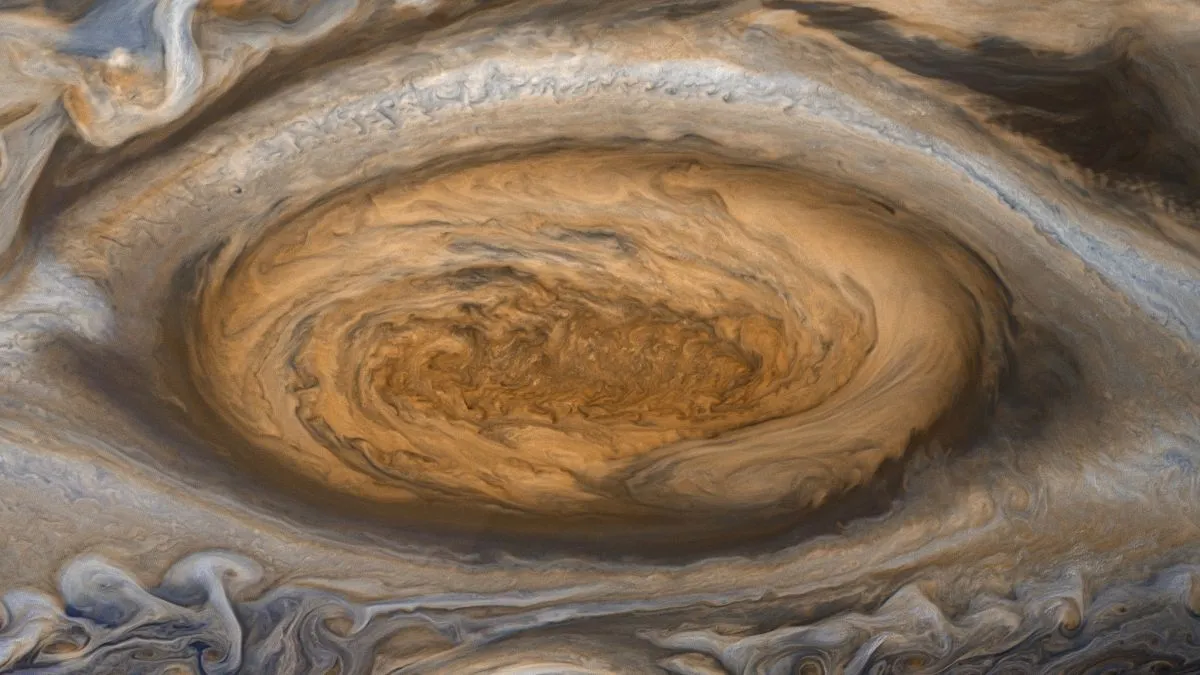
\includegraphics[width=\textwidth]{chp02_background/figures/red_spot.png}
			\caption{Jupiter's Great Red Spot, as photographed by the Voyager probe in 1979 (NASA/JPL-Caltech).}
		\end{subfigure}
		\begin{subfigure}{0.49\textwidth}
			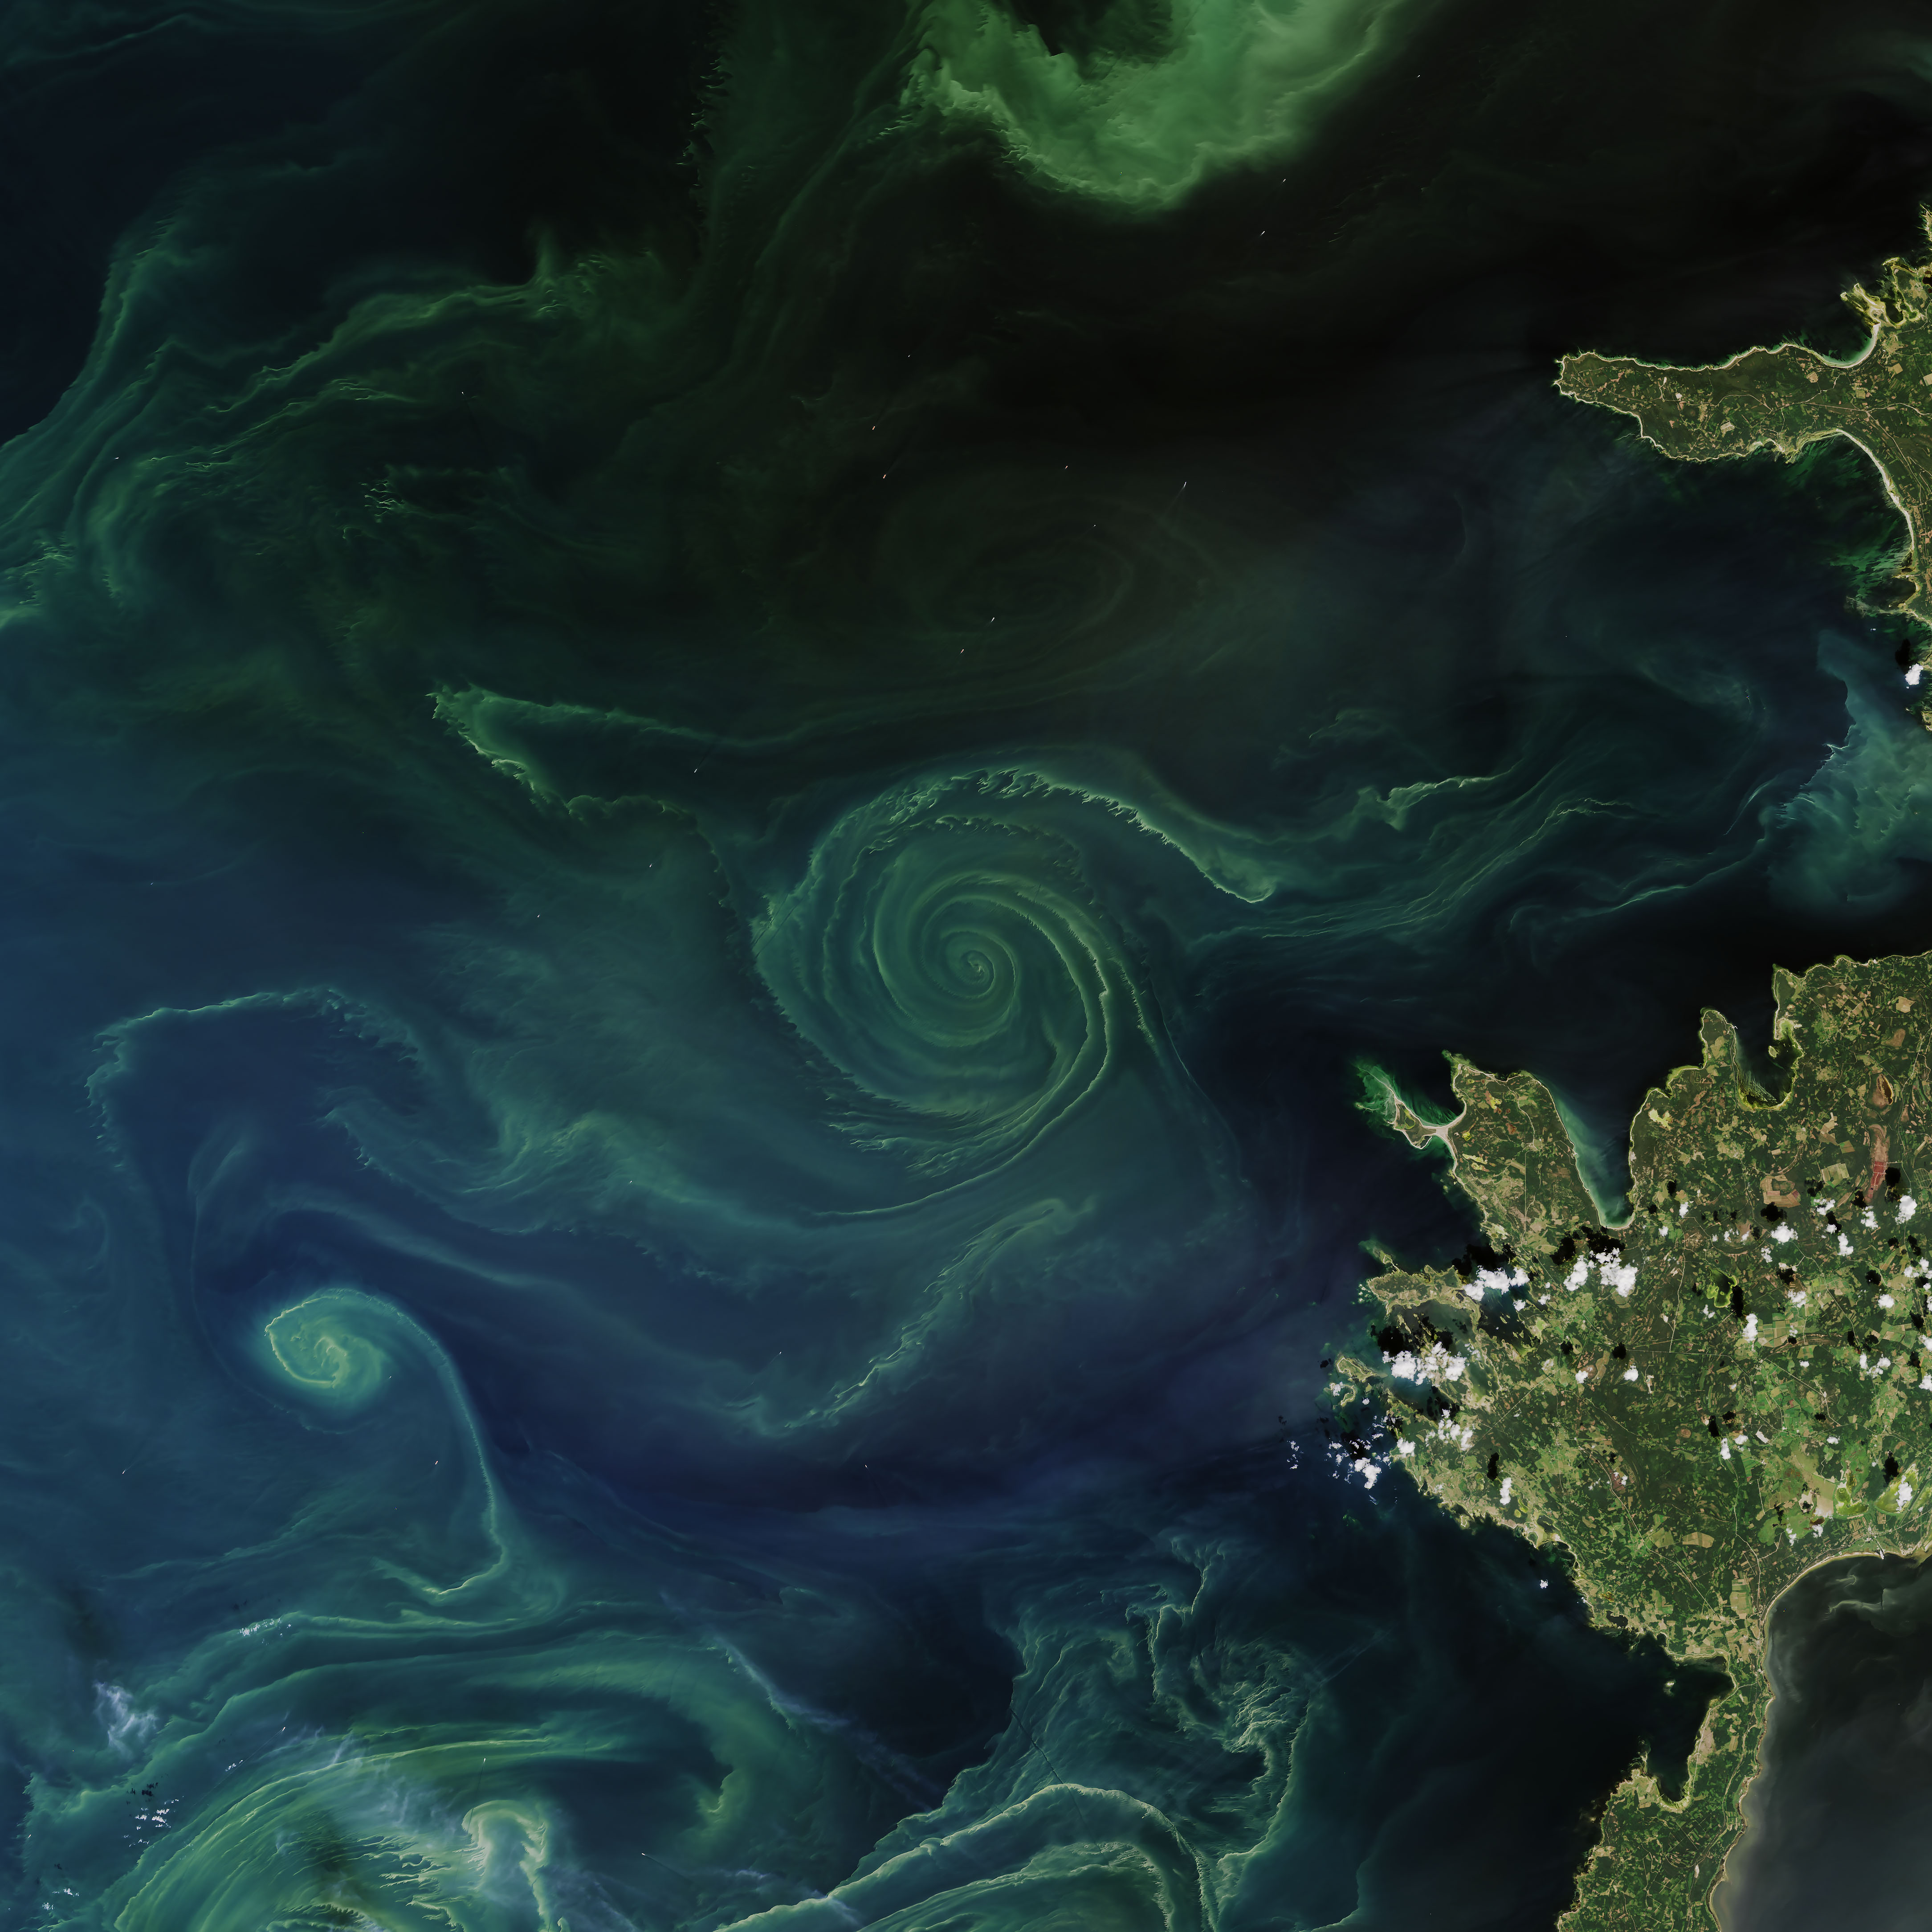
\includegraphics[width=\textwidth]{chp02_background/figures/photoplankton}
			\caption{Photoplankton blooms in the Baltic sea.}
		\end{subfigure}
		\begin{subfigure}{0.49\textwidth}
			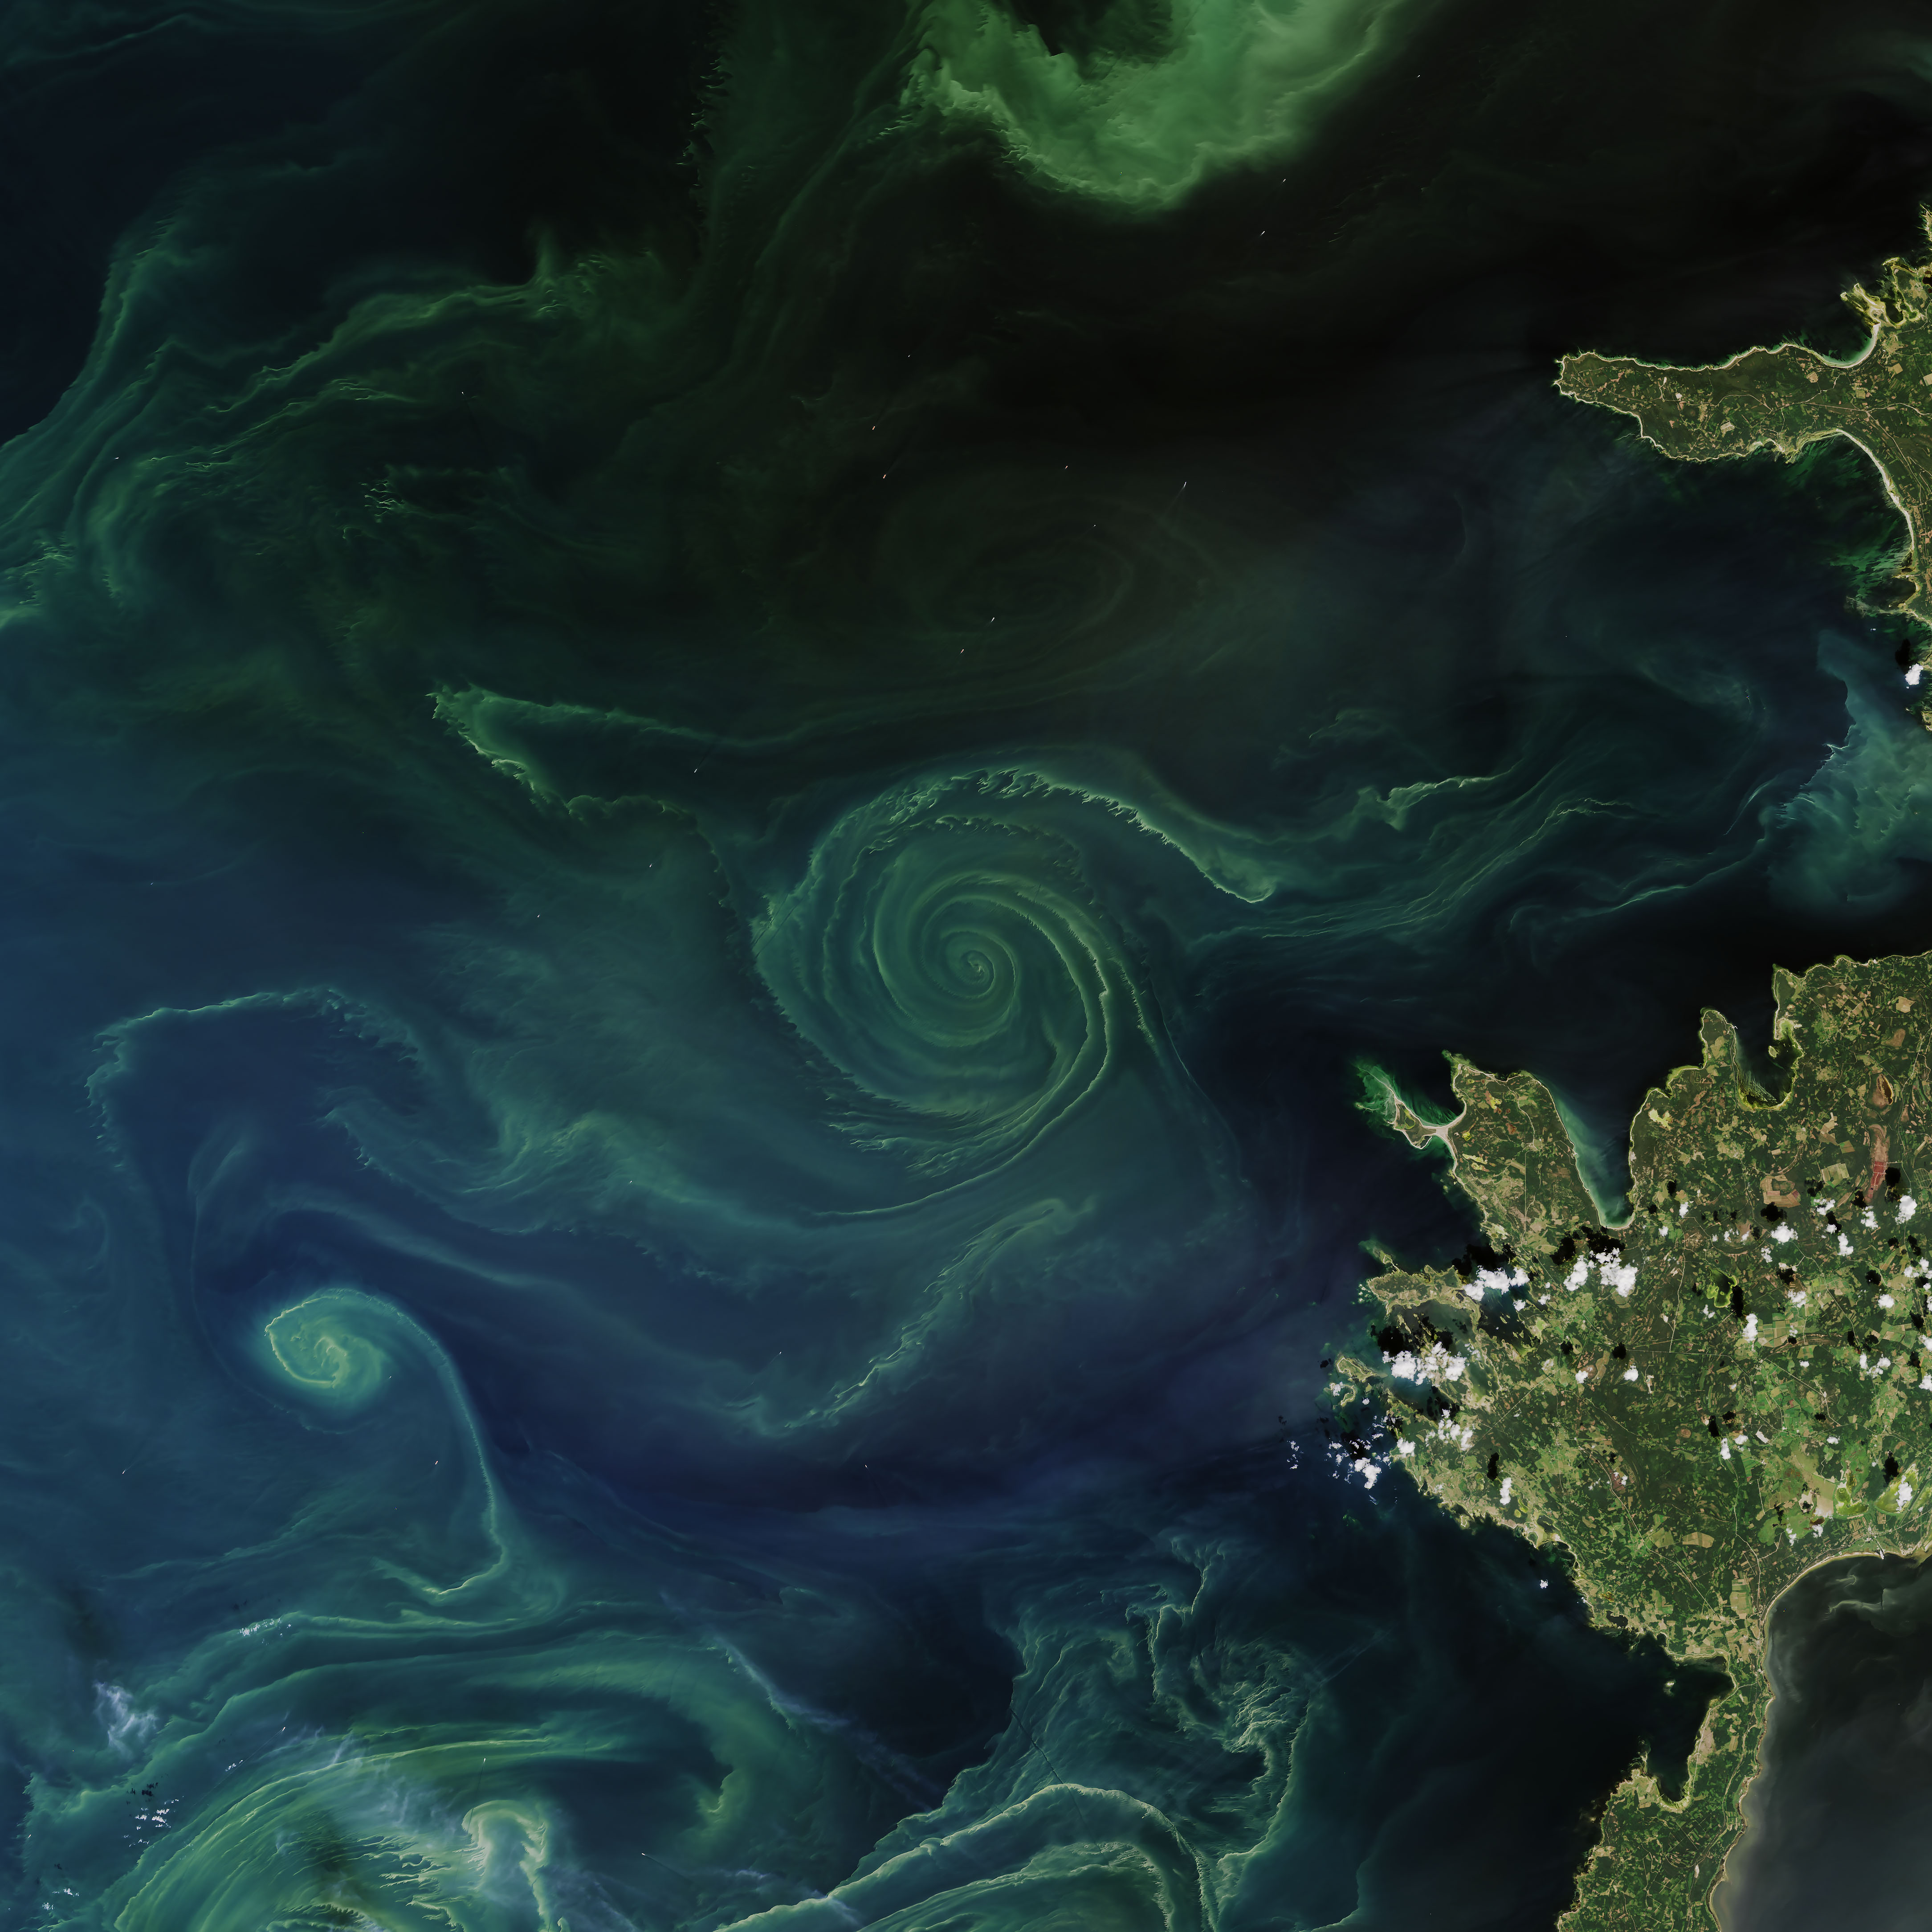
\includegraphics[width=\textwidth]{chp02_background/figures/photoplankton}
			\caption{Photoplankton blooms in the Baltic sea.}
		\end{subfigure}
		\caption{Examples of coherent patterns emerging in fluid flows.}
		\label{fig:lcs_examples}
	\end{center}
\end{figure}

In a steady system (that is, the vector field \(u\) in \cref{eqn:det_ode} is independent of time), we can gain this insight by using classical methods in dynamical systems, such as phase portrait analysis and identifying unstable and stable manifolds.
For example, unstable and stable manifolds cannot be intersected by solution trajectories, and so can act as barriers for the transport of material within a flow.
However, when the system is non-autonomous (that is, the vector field explicitly depends on time \(t\)), these structures can themselves vary with time and the problem of identifying them is far more non-trivial.
Lagrangian coherent structure (LCS) theory provides a mathematical framework for defining and identifying such structures within a given flow \citep{BalasuriyaEtAl_2018_GeneralizedLagrangianCoherent}.

There are many procedures and heuristics for extracting these regions from a given flow, which draw upon different mathematical techniques, including , , and statistical clustering.
Detailed reviews of approaches to Lagrangian coherent structure extraction are provided by \citet{BalasuriyaEtAl_2018_GeneralizedLagrangianCoherent}, \citet{HadjighasemEtAl_2017_CriticalComparisonLagrangian}, and \citet{PeacockDabiri_2010_IntroductionFocusIssue}.

One of the best known procedures for extracting LCSs is via the finite-time Lyapunov exponent (FTLE) \citep{ShaddenEtAl_2005_DefinitionPropertiesLagrangian}, which is a measure quantifying the stretching of infinitesimal regions of a flow over a finite time period.
Take an initial condition \(x\) and let \(F_0^t\) represent the flow map of our system over the time interval \([0,t]\).
We wish to quantify the impact of a small change in the initial condition on the flow at time \(t\), so take \(\delta\) as a small and arbitrary perturbation to \(x\).
Then, we measure the \emph{stretching} in the direction of \(\delta\) with
\[
	s\!\left(x, \delta\right) = \frac{\norm{F_0^t\!\left(x + \delta\right) - F_0^t\!\left(x\right)}}{\norm{\delta}}
\]
For sufficiently small \(\delta\), we can replace the mapped perturbation with a linearisation of the flow map about \(x\), that is
\[
	s\!\left(x, \delta\right) \approx \frac{\norm{\nabla F_0^t\!\left(x\right) \delta}}{\norm{\delta}}.
\]
% \Cref{fig:ftle_illustr} provides a pictorial representation of this calculation; a small !!!!!
Taking the supremum over all possible perturbations \(\delta\), we have
\[
	\sup_{\delta \in \R^n, \, \delta \neq 0}s\!\left(x, \delta\right) \approx \norm{\nabla F_0^t\!\left(x\right)},
\]
which quantifies the stretching about the trajectory \(F_0^t\!\left(x\right)\).
The finite-time Lyapunov exponent is then computed as
\begin{equation}
	\mathrm{FTLE}_0^t\!\left(x\right) = \frac{1}{\abs{t}}\ln\!\left(\norm{\nabla F_0^t\!\left(x\right)}\right).
	\label{eqn:ftle_defn}
\end{equation}
Note that the operator norm \(\norm{\nabla F_0^t\!\left(x\right)}\) in \cref{eqn:ftle_defn} can be readily computed as the square root of the largest eigenvalue of the Cauchy-Green tensor \(\left[\nabla F_0^t\!\left(x\right)\right]^{\T}\nabla F_0^t\!\left(x\right)\).
Over the set of initial conditions, the FTLE is a scalar field.
It was shown by \citet{ShaddenEtAl_2005_DefinitionPropertiesLagrangian} that the maximising ridges of the FTLE field can correspond to flow barriers, and so by finding these ridges, one can extract coherent structures for the flow.
\td{Talk about how FTLE provides general insight into the system too}

% In \Cref{fig:gs_lcs}, we compute the FTLE field of our Gulf Stream velocity model over a timespan of 7 days.



% \begin{figure}
% 	\begin{center}
% 		\begin{subfigure}{0.49\textwidth}
% 			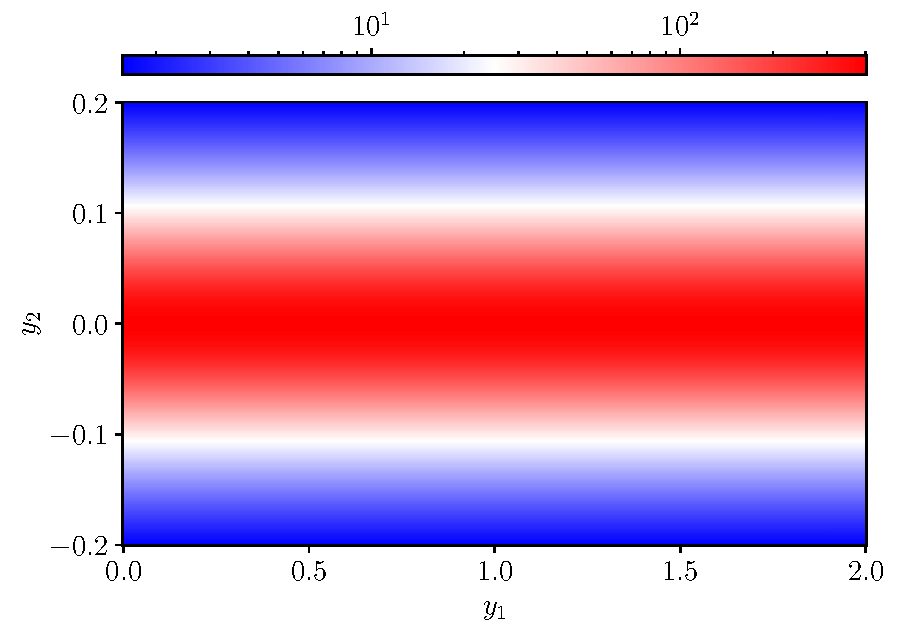
\includegraphics[width=\textwidth]{chp02_background/figures/gulf_stream_motivation/ftle.pdf}
% 			\caption{The finite-time Lyapunov exponent field.}
% 		\end{subfigure}
% 		\begin{subfigure}{0.49\textwidth}
% 			\caption{Maximising ridges of the FTLE field.}
% 		\end{subfigure}
% 		\caption{The finite-time Lyapunov exponent field computed, and corresponding maximising ridges.
% 			This is an example of using a scalar field to extract Lagrangian coherent structures from a fluid flow.
% 			The resulting maximises ridges indicate a skeleton of the Gulf Stream.}
% 		\label{fig:gs_lcs}
% 	\end{center}
% \end{figure}


Most well-established LCS frameworks and extraction procedures are purely deterministic, in that they are defined and compute solely in terms of the behaviour of the underlying ordinary differetnial equation.
However, uncertainty in such systems is inevitable and these methods do not explicitly account for this.
There is accordingly an emerging interest \citep{Balasuriya_2020_StochasticApproachesLagrangian,anymore?} in extending LCS theory to stochastic settings (which is the relevance of LCSs to this thesis).
There are several different ways in which stochasticity is being accounted for in recent LCS developments:
\begin{romanate}
	\item in creating novel computable measures that explicitly account for such ongoing uncertainty, e.g. see (in \Cref{sec:s2_summ}) stochastic sensitivity introduced by \citet{Balasuriya_2020_StochasticSensitivityComputable}, model sensitivity introduced by \citet{KaszasHaller_2020_UniversalUpperEstimate}, and the finite-time divergence rate by \citet{BranickiUda_2023_PathBasedDivergenceRates}.
	These are scalar fields defined on initial conditions that measure the certainty in the corresponding deterministic trajectories, and can be used to extract coherent regions in similar ways to deterministic methods.

	\item in directly extracting coherent regions for the stochastic flow.
	\citet{BalasuriyaGottwald_2018_EstimatingStableUnstable} consider stationary flows subject to small-scale stochastic perturbations, and quantify the behaviour of particles
	\citet{DennerEtAl_2016_ComputingCoherentSets} directly compute coherent sets by working with a discretised Fokker-Planck equation.
	\td{Do a touch more reading on this.}

	\item in understanding the direct impact of velocity uncertainty on well-established deterministic LCS measures.
	\citet{BadzaEtAl_2023_HowSensitiveAre} provide a systematic analysis, using Monte Carlo simulation and summary statistics to evaluate the robustness of several common LCS extraction schemes to velocity uncertainty.
	It is shown that LCS methods that directly account for this uncertainty, such as stochastic sensitivity \citep{Balasuriya_2020_StochasticSensitivityComputable}, are the most robust.
	The finite-time Lyapunov exponent has received particular attention, with recent studies aiming to quantify the impact of velocity field uncertainty on the FTLE computation: \citet{GuoEtAl_2016_FiniteTimeLyapunovExponents} use stochastic simulation and statistical analysis, \citet{Balasuriya_2020_UncertaintyFinitetimeLyapunov} provides theoretical error bounds on the FTLE computation, and \citet{YouLeung_2021_ComputingFiniteTime} propose an approach for computing the expected FTLE field.

\end{romanate}
In this thesis, we are primarily interested point (i), by exploring how our characterisations of uncertainty can be applied to extract coherent structures.
This is directly extending the stochastic sensitivity of \citet{Balasuriya_2020_StochasticSensitivityComputable}, which is summarised in \Cref{sec:s2_summ}.
We will also discuss (in \Cref{ch:outlook}) how we anticipate our work could be applied to point (iii), as a quantification of uncertainty in computations involving the flow map in other LCS schemes.






\section{Stochastic sensitivity}\label{sec:s2_summ}
To conclude our background and motivation, this section provides a brief summary of stochastic sensitivity, a computable measure of uncertainty in flows introduced by \citet{Balasuriya_2020_StochasticSensitivityComputable}.
These tools were provided for 2-dimensional systems only, and the primary motivation was top undestand uncertainty in fluid flows.
% Further technical details, including the main theorems, are reproduced in \Cref{app:s2_details}.

Given possibly time-dependent velocity data \(u: \R^2 \times [0,T] \to \R^2\), \citet{Balasuriya_2020_StochasticSensitivityComputable} considers the evolution of solutions to the differential equation
\begin{equation}\label{eqn:s2_ode}
	\dod{x_t}{t} = u\!\left(x_t, t\right).
\end{equation}
The velocity field \(u\) is \emph{Eulerian}, in that it describes the fluid velocity at a given point in space and time.
The trajectories that solve \cref{eqn:s2_ode} are \emph{Lagrangian}, and correspond to the movement of idealised infinitesimal particles within the flow.
These Lagrangian trajectories are summarised by the flow map \(F_s^t\) of \cref{eqn:s2_ode}.
In most practical situations, the Eulerian velocity data driving ocean and atmospheric models relies upon measurements of estimates obtained on a low resolution spatial discretisation.
\citet{Balasuriya_2020_StochasticSensitivityComputable} introduces stochastic sensitivity as a new tool for directly quantifying the impact of Eulerian uncertainty on Lagrangian trajectories.

To directly account for these unresolved sources of uncertainty, the ``true'' Lagrangian trajectories evolve as solution to the stochastic differential equation
\begin{equation}
	\sde{y_t}{u\left(y_t, t\right)}{\epsilon\sigma\left(y_t, t\right)}, \quad y_0 = x_0
	\label{eqn:s2_sde},
\end{equation}
where \(0 < \epsilon \ll 1\) is a parameter quantifying the scale of the noise, \(\sigma:	\R^2\times[0,T] \to \R^{2\times 2}\) is the \(2\times 2\) diffusion matrix, and \(W_t\) is the canonical two-dimensional Wiener process.
In the original formulation \citep{Balasuriya_2020_StochasticSensitivityComputable}, \(\epsilon\) is a dimensionless parameter and \(\sigma\) is dimensional, but an alternative scaling technique relates \(\epsilon\) to spatial and velocity uncertainty scales in the data (see the follow-up work by \citet{BadzaEtAl_2023_HowSensitiveAre,Balasuriya_2020_UncertaintyFinitetimeLyapunov,FangEtAl_2020_DisentanglingResolutionPrecision} for examples).
Since \(\sigma\) can vary by both space and time, the noise is permitted to be multiplicative.
The diffusion matrix \(\sigma\) is specified \emph{a priori}, based on any knowledge of how uncertainty varies with space and time, e.g. from experimental considerations, observation error estimates.
If no such prior information is known, then \(\sigma \equiv I\), the \(2 \times 2\) identity matrix is the default choice.
The SDE \cref{eqn:s2_sde} is considered subject to a \emph{fixed} initial condition \(x_0\).

To quantify uncertainty in a way that is independent of the noise scale \(\epsilon\), \citet{Balasuriya_2020_StochasticSensitivityComputable} defined the random variable \(z_\epsilon\left(x_0,t\right)\) as
\[
	z_\epsilon\!\left(x_0,t\right) \coloneqq \frac{y_t - F_0^t(x_0)}{\epsilon},
\]
which captures the random deviation between the ``true'' stochastic trajectories and the deterministic flow map.
The aim was to compute statistics of \(z_\epsilon\).
To derive such quantities that can be computed in practice, \citet{Balasuriya_2020_StochasticSensitivityComputable} considers the signed projection of \(z_\epsilon\!\left(x,t\right)\) onto a ray emanating from the deterministic position \(F_0^t(x)\) in a given direction \(\theta\), defining
\[
	P_\epsilon\!\left(x,\theta\right) \coloneqq \hat{n}^{\T}\!\left(\theta\right) z_\epsilon\!(x_0,t), \quad \hat{n}\!\left(\theta\right) = \begin{bmatrix}
		\cos{\theta} \\
		\sin{\theta}
	\end{bmatrix}.
\]
where \(\theta \in \left[-\pi/2, \pi/2\right)\).
The statistics of \(z_\epsilon\left(x,T\right)\) and \(P_\epsilon(x,\theta)\) are considered in the limit as \(\epsilon\downarrow 0\), which provides a characterisation of the uncertainty of the model that is \emph{independent} of the scale of the noise.
\citet{Balasuriya_2020_StochasticSensitivityComputable} provided computable expressions for the mean and variance of \(P_\epsilon\left(x,\theta\right)\) in this limit of small noise, which we summarise here.
For proofs of these results, see the appendices of \citet{Balasuriya_2020_StochasticSensitivityComputable}.

\begin{definition}[\citealt{Balasuriya_2020_StochasticSensitivityComputable}]
	\begin{alpharate}
		\item The \textbf{anisotropic uncertainty} is a scalar field \(A: \R^2\times\left[-\pi/2, \pi/2\right) \to [0,\infty)\) defined by
		\[
			A(x,\theta) \coloneqq \sqrt{\lim_{\epsilon\downarrow 0}\var{P_\epsilon(x,\theta)}}.
		\]

		\item The \textbf{stochastic sensitivity} is a scalar field \(S: \R^2 \to [0,\infty)\) defined by
		\[
			S^2(x) \coloneqq \lim_{\epsilon\downarrow 0}\sup_{\theta}{\var{P_\epsilon(x,\theta)}}.
		\]
	\end{alpharate}
\end{definition}

The anisotropic uncertainty is a measure of the uncertainty in a specified direction \(\theta\), whereas stochastic sensitivity is a scalar field which for a given initial condition measures the uncertainty in the corresponding Lagrangian trajectory.
By employing techniques from both deterministic and stochastic calculus (i.e. Gr\"onwall's inequality, the Burkholder-Davis-Gundy inequality, It\^o's Lemma), \citet{Balasuriya_2020_StochasticSensitivityComputable} further established expressions for both the anisotropic uncertainty and the stochastic sensitivity that are computable given only the flow map and velocity data.

\begin{theorem}[\citealt{Balasuriya_2020_StochasticSensitivityComputable}]\label{thm:orig_s2_calculation}
	For \(x \in \R^2\), set \(w \coloneqq F_0^t(x)\).
	Then, for any \(\theta \in \left[-\pi/2, \pi/2\right)\),
	\[
		A\!\left(x,\theta\right) = \left(\int_0^T{\norm{\Lambda\left(x, t, T\right)J\hat{n}\!\left(\theta\right)}\dif t}\right)^{1/2},
	\]
	where
	\td{Use \(w\) appropriately}
	\[
		\Lambda\!\left(x,t\right) \coloneqq e^{\int_t^T{\left[\nabla \cdot u\right]\left(F_t^\xi\!\left(x\right), \xi\right)\dif\xi}}\sigma\left(F_0^t(x), t\right)^{\T}J \nabla_w F_T^t\!\left(w\right),
	\]
	with the gradients \(\nabla_w\) of the flow map taken with respect to the mapped position \(w\), and
	\[
		J \coloneqq \begin{bmatrix}
			0 & -1 \\
			1 & 0
		\end{bmatrix}
	\]
	Additionally, stochastic sensitivity is computed as
	\[
		S^2(x) = P(x) + N(x),
	\]
	with
	\begin{align*}
		L(x) & \coloneqq \frac12\sum_{i=1}^2\int_0^T\left[\Lambda_{i2}\left(x,t, T\right)^2 - \Lambda_{i1}\left(x,t,T\right)^2\right]\dif t \\
		M(x) & \coloneqq \sum_{i=1}^2\int_0^T{\Lambda_{i1}\left(x,t,T\right)\Lambda_{i2}\left(x,t,T\right)\dif t}                           \\
		N(x) & \coloneqq \sqrt{L^2(x) + M^2(x)}                                                                                             \\
		P(x) & \coloneqq \abs{\frac12\sum_{i=1}^2\sum_{j=1}^2{\int_0^T{\Lambda_{ij}\left(x,t,T\right)^2\dif t}}},
	\end{align*}
	where \(\Lambda_{ij}\) is the \((i,j)\)-element of \(\Lambda\).
\end{theorem}



A \emph{robust set} is a subset of initial conditions such that the stochastic sensitivity is below a given threshold.
That is, a robust set consists of those initial conditions for which the uncertainty in the corresponding flow trajectory, as measured by stochastic sensitivity, is small enough.



\subsection{Current applications \& shortcomings}
Since stochastic sensitivity is only a recent development, it has only been applied in a limited number of places so far.
Here, we briefly review the literature in which the original formulation stochastic sensitivity by \citet{Balasuriya_2020_StochasticSensitivityComputable} has been applied.

\begin{itemize}
	\item \citet{Balasuriya_2020_UncertaintyFinitetimeLyapunov} uses stochastic sensitivity to compute an error bound for the finite-time Lyapunov (FTLE) computation.
	      The computable \(S^2\) value is used as an estimate of the standard deviation of the deviation between the deterministic and ``true'' (stochastic) trajectories, leading to a computable error bound on the FTLE value.


	\item \citet{FangEtAl_2020_DisentanglingResolutionPrecision}


	\item \citet{BadzaEtAl_2023_HowSensitiveAre} investigate the impact of velocity uncertainty on Lagrangian coherent structures (e.g. see the reviews by \citet{BalasuriyaEtAl_2018_GeneralizedLagrangianCoherent} and \citet{HadjighasemEtAl_2017_CriticalComparisonLagrangian}) extracted as robust sets with stochastic sensitivity.
	      The stochastic model \cref{eqn:ss_sde} is used to generate realisations of Lagrangian trajectories subject to noise on the velocity field.
	      By directly capturing such uncertainty as a means of coherent set \citet{BadzaEtAl_2023_HowSensitiveAre} showed that robust sets extracted with stochastic sensitivity do SOMETHING.

\end{itemize}
There are several limitations to the work as originally presented by \citet{Balasuriya_2020_StochasticSensitivityComputable}:
\begin{enumerate}
	\item The tools are restricted to two-dimensional models, and the constructions using projections have no obvious extension to \(n\)-dimensions.
	      Extending stochastic sensitivity to \(n\)-dimensions will enable application to a much broader class of models beyond the fluid flow context, including high-dimensional climate models.

	\item \citet{Balasuriya_2020_StochasticSensitivityComputable} only computes the expectation and variance of the projections \(P_\epsilon(x,\theta)\), which does not give us the distribution under the limit as \(\epsilon\) approaches 0.

	\item The computational formula for the anisotropic uncertainty and stochastic sensitivity, as described in \Cref{thm:orig_s2_calculation}, require knowledge of the divergence \(\nabla\cdot u\) of the velocity field, and computation of four integrals.
\end{enumerate}



In \Cref{sec:theory_s2}, we present an extension of stochastic sensitivity to \(n\)-dimensions that overcomes these limitations.
